\section{Evaluation Results} \label{sec:evaluation-results}

This section presents and discusses the results of our evaluation.
\Cref{sec:establishing-baseline-performance} establishes a baseline for the subsequent results comparison.
The discussion then pivots to \textbf{\ac{RT} 3}, delving into the identification of optimal feature weights for the Citation Recommender and pinpointing the most effective language model for the Language Recommender. These are elaborated upon in \Cref{sec:evaluation-citation-recommender} and \Cref{sec:evaluation-language-recommender}, respectively.
Finally, \Cref{sec:evaluation-hybrid-recommender} addresses \textbf{\ac{RT} 4} by comparing the two hybridization orders in terms of \ac{MAP} and recommendation diversity and analyzing the interactions between the Citation Recommender and the Language Recommender.


\subsection{Establishing a Baseline Performance} \label{sec:establishing-baseline-performance}

To contextualize \ac{MAP} scores of various feature weights and language models, a baseline performance is needed.
This baseline is established by constructing a \emph{Null Model} that randomly selects papers from the training set as recommendations.

In contrast to the Precision metric, where the baseline performance can be easily determined analytically, the \ac{MAP} requires a simulation-based approach.
This approach involves sampling recommendation lists filled with 0s (irrelevant) and 1s (relevant) at random and computing the \ac{AP} for each list.
The baseline \ac{MAP} is derived from averaging these \ac{AP} values across all simulation runs.
Two parameters influence the simulation results: the number of recommendations for each run and the probability of drawing a relevant item.
\Cref{tab:baseline-map} presents simulation results for various combinations of these parameters.

\begin{table}[htb!]
    \centering
    \begin{tabular}{ccc}
        \toprule
        \textbf{0/1 Ratio}          & \textbf{\# Recommendations} & \textbf{MAP}   \\
        \midrule
        20/80                       & 10                          & 0.843          \\
        20/80                       & 20                          & 0.828          \\
        20/80                       & 50                          & 0.815          \\
        50/50                       & 10                          & 0.608          \\
        50/50                       & 20                          & 0.569          \\
        50/50                       & 50                          & 0.536          \\
        71.3/28.7                   & 10                          & 0.433          \\
        \textbf{71.3}/\textbf{28.7} & \textbf{20}                 & \textbf{0.384} \\
        71.3/28.7                   & 50                          & 0.338          \\
        80/20                       & 10                          & 0.350          \\
        80/20                       & 20                          & 0.308          \\
        80/20                       & 50                          & 0.257          \\
        \bottomrule
    \end{tabular}
    \caption[Baseline \acs{MAP} Scores]{\ac{MAP} for simulated recommendation lists. Each list contains binary values: 0 for irrelevant and 1 for relevant recommendations. The samples are randomly drawn from a Bernoulli distribution.
        The first column displays the proportions of irrelevant and relevant items, or, equivalently, the probability $p$ of the Bernoulli distribution to draw a relevant item.
        The second column indicates the length of the recommendation list, and the third column the resulting \ac{MAP}. The bold values highlight the parameters for the Null Model baseline in this thesis. Generally, the \ac{MAP} increases with a higher proportion of relevant items but decreases with a higher number of recommendations.}
    \label{tab:baseline-map}
\end{table}

The simulation parameters for this thesis's evaluation are based on the properties of the test set.
Thus, the probability of sampling a relevant candidate is set to $0.287$, which corresponds to the average fraction of relevant query papers in the test set.
The number of recommendations is set to $20$, which is the default number of recommendations for the hybrid system.
According to these parameters, we simulate $100,000$ recommendation rankings and calculate the \ac{AP} for each, yielding a baseline \ac{MAP} of $0.384$.


\subsection{Evaluating the Citation Recommender} \label{sec:evaluation-citation-recommender}

The evaluation strategy presented in \Cref{sec:evaluation-strategy} identified feature weight ranges of $[0, 20]$ for the publication date, document citation count, and author citation count, and $[0, 100]$ for the co-citation analysis and bibliographic coupling features.
As the ranges for the citation-based features were adjusted to include higher values than the ranges for the global document characteristics, the citation-based features exert a more substantial influence on recommendation performance.

\Cref{fig:feature-weights-evaluation} shows the \ac{MAP} values for the Citation Recommender candidates averaged over all query papers in the test set.
The y-axis displays the selected weight candidates from step 2 of the evaluation process. The integer values correspond to the order [publication date, document citation count, author citation count, co-citation analysis, and bibliographic coupling].

\begin{figure}[htb!]
    \centering
    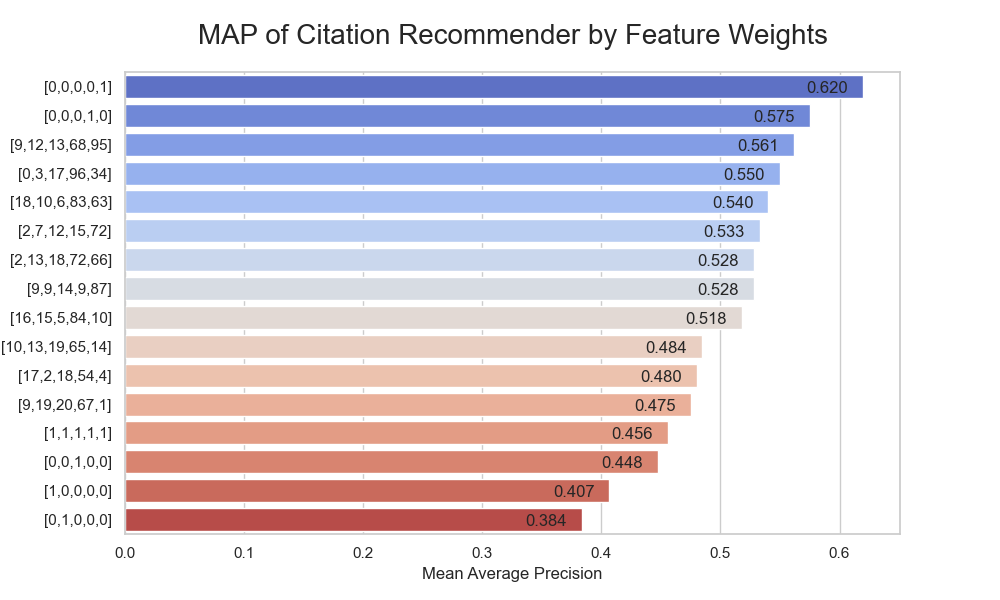
\includegraphics[width=\textwidth]{plots/feature_weights.png}
    \caption[Feature Weights Evaluation]{Performance evaluation of the Citation Recommender using different feature weights. The y-axis shows the feature weights for the publication date, document citation count, author citation count, co-citation analysis, and bibliographic coupling in that order. The x-axis shows the \ac{MAP} values for the Citation Recommender candidates averaged over all query papers in the test set. Larger weights for the co-citation analysis and bibliographic coupling scores generally lead to higher \ac{MAP} values.
        Bibliographic coupling performs best with a \ac{MAP} of $0.620$, whereas the worst performing feature is the paper citation count with a \ac{MAP} of $0.384$.
    }
    \label{fig:feature-weights-evaluation}
\end{figure}

The bibliographic coupling weight varies heavily among the top 10 candidates, taking on high values like $95$ or $87$ in some instances and lower values like $1$ or $4$ in others.
A similar pattern can be observed for the co-citation analysis weight, though its variation is slightly less pronounced. The weights for the publication date, document citation count, and author citation count spread fairly evenly within their $[0, 20]$ range.

\Cref{fig:feature-weights-evaluation} indicates significant performance differences across different weight vectors.
For instance, the lowest \ac{MAP} of $0.384$ is achieved by the vector $[0, 1, 0, 0, 0]$ isolating the paper citation count, while the highest \ac{MAP} of $0.620$ is observed for $[0, 0, 0, 0, 1]$, which puts the full weight on the bibliographic coupling score.
In contrast, the vectors with full weight on the global document features indicate the worst performance. Using only the paper citation count to generate recommendations yields a \ac{MAP} of $0.384$, which is exactly equal to the baseline \ac{MAP} of the Null Model. This suggests that, averaged over all query papers in the test set, selecting the most cited papers is not more effective than the random selection of arbitrary papers from the training set.

Weight vectors identified by the randomized search predominantly lead to good but not great results. They range from a \ac{MAP} of $0.475$ for the weights $[9, 19, 20, 67, 1]$ to a \ac{MAP} of $0.561$ for the vector $[9, 12, 13, 68, 95]$.
In line with prior observations, we can identify the general trend that higher weights for the bibliographic coupling and co-citation analysis features lead to higher \ac{MAP} values.
A potential reason that weight vectors found by the randomized search do not generalize well to the test set is that the candidate selection process optimized for the Hybrid Recommender performance (averaging the \ac{MAP} scores of the \ac{C2L} and \ac{L2C} orders) rather than for the Citation Recommender performance.
In \Cref{fig:feature-weights-evaluation}, only the latter is portrayed.


\subsection{Evaluating the Language Recommender} \label{sec:evaluation-language-recommender}

To identify the optimal language model for the Language Recommender, \Cref{tab:language-recommender-evaluation} shows the \ac{MAP} values for the Language Recommender candidates averaged over all query papers in the test set.

\begin{table}[htb!]
    \centering
    \begin{tabular}{lc}
        \toprule
        \textbf{Language Model} & \textbf{MAP}   \\
        \midrule
        TF-IDF                  & 0.628          \\
        BM25                    & 0.596          \\
        Word2Vec                & 0.588          \\
        FastText                & 0.575          \\
        GloVe                   & 0.581          \\
        BERT                    & 0.603          \\
        \textbf{SciBERT}        & \textbf{0.660} \\
        Longformer              & 0.524          \\
        \bottomrule
    \end{tabular}
    \caption[Evaluation of the Language Recommender]{Performance evaluation of the Language Recommender candidates using different language models. The \ac{MAP} per language model is calculated by averaging over all query papers in the test set. Models with similar properties tend to produce similar results. The SciBERT model, highlighted in bold, achieves the highest \ac{MAP} of $0.660$. The Longformer model performs worst with a \ac{MAP} of $0.524$.}
    \label{tab:language-recommender-evaluation}
\end{table}

The SciBERT model achieves the highest \ac{MAP} score of $0.660$, with TF-IDF and BERT following at $0.628$ and $0.603$, respectively. The Longformer model performs worst with a \ac{MAP} of $0.524$. Comparing the findings with \Cref{fig:feature-weights-evaluation}, it is evident that the Language Recommender candidates outperform the Citation Recommender candidates. This suggests that processing paper abstracts with language models is generally more effective for paper recommendation than relying on global document characteristics and citation-based features.

However, the performance differences between Citation Recommender and Language Recommender can diminish depending on which feature weights and language model are selected.
For example, the Citation Recommender with the weight vector $[0, 0, 0, 0, 1]$ outperforms the Language Recommender for 6 of the 8 language models with a \ac{MAP} of $0.620$. Conversely, the Language Recommender employing the Longformer model only ranks ninth out of 16 within the feature weights ranking of the Citation Recommender.
Nonetheless, the Language Recommender produces more robust and reliable results. Even its lowest \ac{MAP} score of $0.524$ significantly surpasses the lowest Citation Recommender score of $0.384$.
In particular, all language models outperform the Null Model baseline by a large margin.

There is a weak correlation between the language model category and recommendation performance. Models that have similar structural characteristics produce comparable results. For instance, the contextual embedding models SciBERT and BERT as well as the sparse embedding models TF-IDF and BM25 all exhibit above-average performance.
Conversely, the static embedding models Word2Vec, FastText, and GloVe all perform below average. The Longformer model is the only outlier, performing worse than all other models despite being a contextual embedding model like BERT and SciBERT.


\subsubsection*{Longformer's Performance}

While the strong performance of SciBERT can be attributed to its domain-specific pretraining on scientific text, the subpar performance of the Longformer model appears surprising at first glance.
The primary aspect that distinguishes Longformer is its design to efficiently process long documents beyond the 512 token limit of BERT by modifying the self-attention mechanism of the Transformer architecture.
Moreover, it is pretrained specifically on a corpus comprising long documents.

However, only $0.58\%$ of all abstracts in the test set exceed the 512 token threshold, implying that the Longformer's advantage over BERT and SciBERT is relevant for only a small fraction of documents.
Due to the discrepancy between the distribution of the pretraining and inference corpora, Longformer's global attention tokens may be optimized for long documents, thereby rendering them less effective for succinct abstracts.
As a result of these disparities, Longformer might allocate more capacity for handling long-range dependencies and might not extract finer local patterns that are crucial for short texts like paper abstracts.

While we are unable to pinpoint a definitive reason for Longformer's poor performance in our evaluations, the underlying factor might even stem from the multitude of parameters that differentiate the Longformer and BERT models, some of which are listed in \Cref{tab:bert_longformer_tokenizer}.
These encompass different tokenizers, optimization techniques, learning rates, weight initialization protocols, or even a discrepancy in the number of training epochs.
To identify the root cause, a methodical approach could involve varying individual parameters sequentially, observing any resulting changes in the recommendation performance.
Given the constraints of computational time and resources, several strategies can be contemplated.

If a full retraining of the Longformer model is feasible, an iterative adaptation of Longformer's and BERT's parameters can be undertaken, including the pretraining corpus, tokenizer, and optimizer, while observing their effect on recommendation performance.
Alternatively, if a full-scale retraining proves impracticable but fine-tuning remains achievable, we might consider fine-tuning the Longformer model using a subset of the paper abstracts. If the performance improves significantly, it indicates that the original pretrained weights are not ideal and differences in the pretraining corpus's characteristics might be the root cause.
In the event that neither exhaustive retraining nor fine-tuning is a viable option, a comparative assessment of the Longformer and BERT models on either extensively long documents, like full paper texts, or very short documents, like paper titles, could be conducted.
A diminished performance disparity for extended documents coupled with an amplified performance gap for short documents would suggest that either the nature of the pretraining corpus or the distinct attention mechanics is the underlying cause of Longformer's poor performance.


\subsection{Evaluating the Hybrid Recommender} \label{sec:evaluation-hybrid-recommender}

Previous sections have focused on the \emph{marginal} performance of the Citation Recommender (\Cref{sec:evaluation-citation-recommender}) and the Language Recommender (\Cref{sec:evaluation-language-recommender}). This section shifts focus to the \emph{interactions} between the two recommenders in the hybrid setup.
Given that the cascade hybridization strategy follows a sequential approach without communication between the two recommenders, it's intuitive that the Citation Recommender and the Language Recommender operate independently.
Subsequent sections investigate whether this assumption holds true.

\Cref{fig:language-models-feature-weights-heatmap-c2l} shows the \ac{MAP} values of the \ac{C2L} Hybrid Recommender for all combinations of feature weights and language models. The first column of the heatmap represents the \ac{MAP} values for the Citation Recommender candidates before re-ranking.

\begin{figure}[htb!]
    \centering
    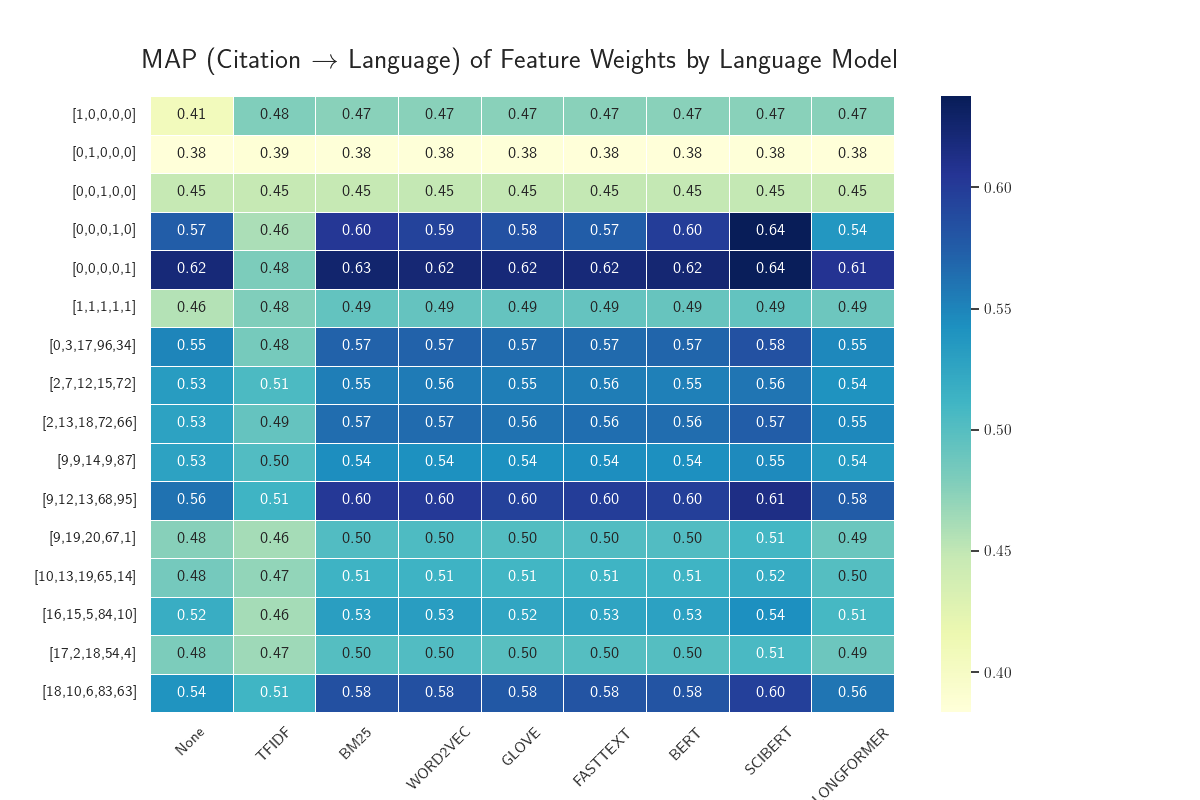
\includegraphics[width=\textwidth]{plots/language_models_feature_weights_heatmap_c_to_l.png}
    \caption[Performance Evaluation of the \acl{C2L} Hybrid Recommender]{Performance evaluation of the \ac{C2L} Hybrid Recommender using various feature weights and language models. Darker colors correspond to higher \ac{MAP} values. The first column presents the \ac{MAP} values for candidates from the Citation Recommender prior to re-ranking. The following columns display \ac{MAP} values after the re-ranking by the Language Recommender using the respective language model for each feature weight vector. SciBERT consistently delivers the highest performance improvements, while TF-IDF is the sole model that generally results in a decrease in \ac{MAP} during re-ranking.}
    \label{fig:language-models-feature-weights-heatmap-c2l}
\end{figure}

To conclude independence between the two recommenders, two conditions must be met:
First, the re-ranking effect of each language model should not depend on the feature weights.
In other words, the column-wise differences to the first column should be constant across all rows.
As this condition compares values within the same column of \Cref{fig:language-models-feature-weights-heatmap-c2l}, we term this condition \emph{vertical independence}.

Second, the relative performance ranking between language models should be the same when the Language Recommender is used for candidate selection (\Cref{tab:language-recommender-evaluation}) and when it is used for re-ranking (\Cref{fig:language-models-feature-weights-heatmap-c2l}).
Thus, we expect the highest \ac{MAP} scores for SciBERT and the lowest for Longformer within each row of the heatmap.
As this condition compares values within the same row of \Cref{fig:language-models-feature-weights-heatmap-c2l}, we term this condition \emph{horizontal independence}.

\Cref{fig:language-models-feature-weights-heatmap-c2l} indicates that vertical independence is not met. The re-ranking effect of each language model varies heavily between the feature weights. For example, none of the language models can improve the candidate recommendations generated with weights $[0,0,1,0,0]$. In contrast, the recommendations for the $[18,10,6,83,63]$ weight vector in the final row can be significantly improved by re-ranking with all language models except TF-IDF.

However, horizontal independence is almost satisfied. With the exception of the TF-IDF model, the most performant candidate selectors (SciBERT, BERT and BM25) are generally also the most performant re-ranking models, indicated by the highest \ac{MAP} values within each row. Conversely, the least performant candidate selector, Longformer, remains the least performant re-ranking model for most feature weight vectors.

A further question of interest is whether high initial \ac{MAP} scores from the Citation Recommender are associated with either a strong or a weak re-ranking effect.
However, \Cref{fig:language-models-feature-weights-heatmap-c2l} reveals no clear relationship between the initial \ac{MAP} scores in the first column and the effect size of re-ranking.
For example, the worst weight vector of $[0,1,0,0,0]$ cannot be improved by re-ranking, while the second to worst weight vector of $[1,0,0,0,0]$ can be significantly improved by re-ranking.
At the higher end of performance, the optimal weight vector $[0,0,0,0,1]$ shows only minimal improvement when re-ranked. In contrast, the second-best weight vector, $[0,0,0,1,0]$, is profoundly influenced by the Language Recommender. Notably, the SciBERT model boosts its \ac{MAP} from $0.57$ to $0.64$.

The heatmap corresponding to the reverse \ac{L2C} ordering is displayed in \Cref{fig:language-models-feature-weights-heatmap-l2c}.
We can observe that feature weight vectors performing poorly for candidate selection (\Cref{fig:feature-weights-evaluation}) also underperform during the re-ranking step. However, this trend does not apply to the top-performing feature weights $[0, 0, 0, 1, 0]$ and $[0, 0, 0, 0, 1]$. These vectors consistently yield worse \ac{MAP} scores in the re-ranking process than weight vectors with a mix of non-zero weights.


\subsubsection*{Inspecting the TF-IDF Behavior}

A striking observation in \Cref{fig:language-models-feature-weights-heatmap-c2l} is the underwhelming performance of the TF-IDF model during re-ranking. Out of the $16$ weight vectors, TF-IDF worsens the recommendations in $12$ cases. In some instances, this decline is dramatic, as evidenced by the drop from $0.62$ to $0.48$ for the weight vector $[0,0,0,0,1]$. This finding is unexpected, given that TF-IDF is the second-best candidate selector, as shown by \Cref{tab:language-recommender-evaluation}. Moreover, given that the second sparse vector embedding model, BM25, does not have this issue, there is no clear methodological explanation for the poor performance of TF-IDF in the hybrid setup. This section further investigates the impact of the TF-IDF model within the hybrid system.

\Cref{fig:tfidf-change-in-map} demonstrates the effect of TF-IDF on the Hybrid Recommender's \ac{MAP} when used for re-ranking (left) or candidate selection (right).
For the \ac{C2L} order, there appears to be a negative correlation between the weights of bibliographic coupling and co-citation analysis and the resulting change in \ac{MAP} from re-ranking:
The greater the weights assigned to these two features, the more the \ac{MAP} decreases after re-ranking with TF-IDF.
The most pronounced performance declines correspond to the weight vectors $[0, 0, 0, 0, 1]$ and $[0, 0, 0, 1, 0]$, where one of the citation-based features is given the full weight of $1$.
In contrast, weight vectors such as $[1, 0, 0, 0, 0]$, $[0, 1, 0, 0, 0]$, and $[0, 0, 1, 0, 0]$, which don't factor in bibliographic coupling and co-citation analysis, and the vector $[1,1,1,1,1]$, with a minimal relative impact from these two features, see improvements from re-ranking.

\begin{figure}[htb!]
    \centering
    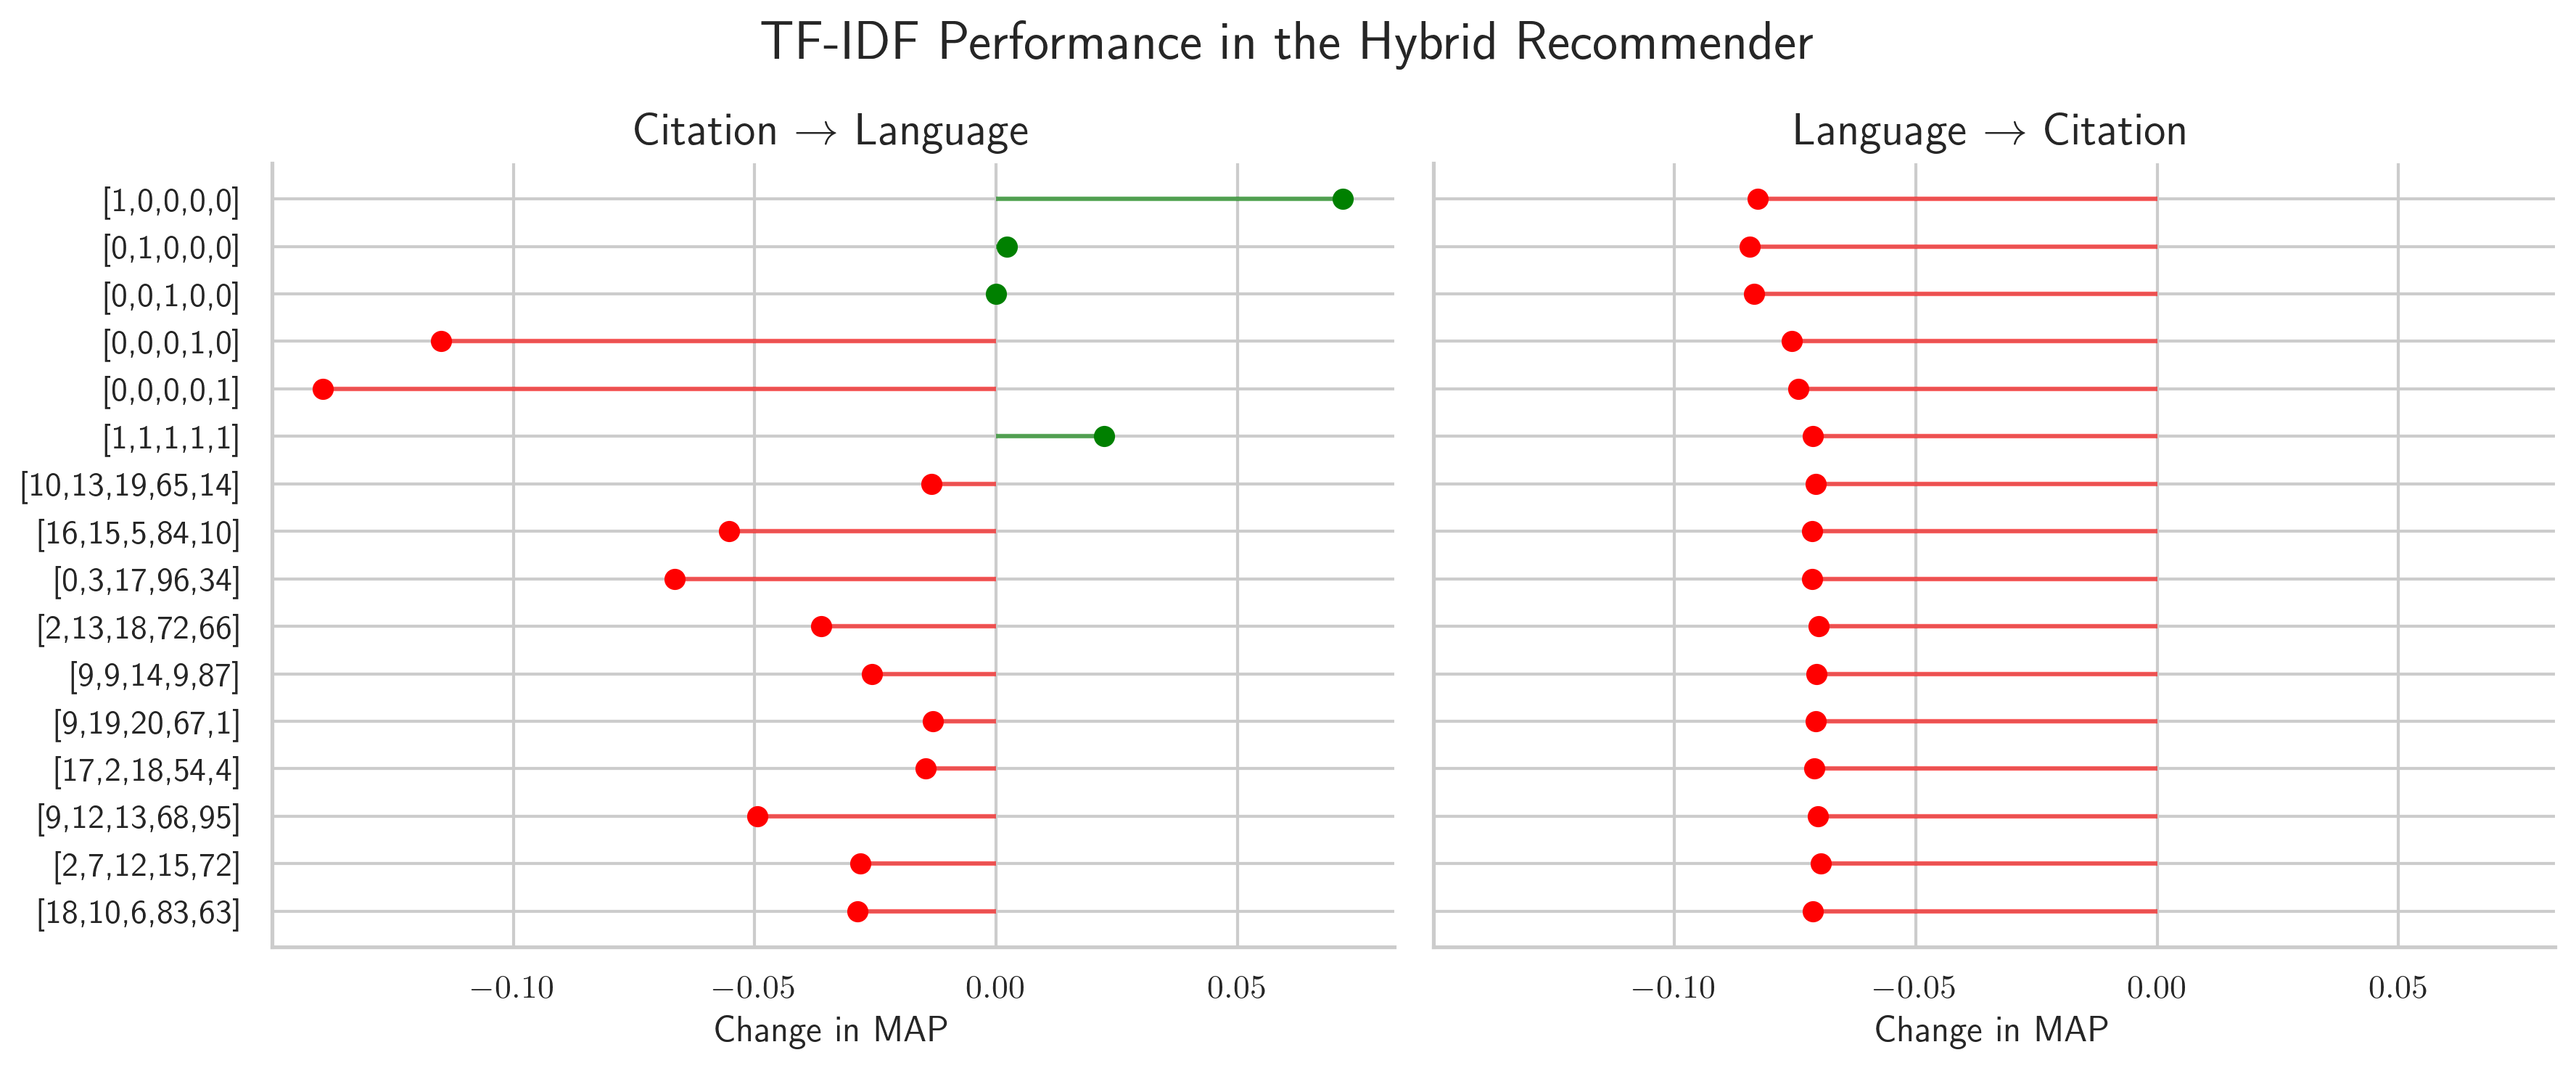
\includegraphics[width=\textwidth]{plots/tfidf_change_in_map.png}
    \caption[Performance of TF-IDF in the Hybrid Recommender]{Performance changes in MAP due to the TF-IDF model. The left plot depicts the MAP change when TF-IDF is employed for re-ranking, whereas the right plot illustrates the MAP change when TF-IDF is utilized for initial candidate selection. The y-axis displays feature weights for the publication date, document citation count, author citation count, co-citation analysis, and bibliographic coupling, respectively. Green lines signify an MAP increase, and red lines denote a decrease. Except for baseline weight vectors with diminished weights for co-citation analysis and bibliographic coupling, TF-IDF generally reduces the MAP during re-ranking. Conversely, when TF-IDF is applied for candidate selection, the Citation Recommender consistently lowers the MAP during the re-ranking phase.}
    \label{fig:tfidf-change-in-map}
\end{figure}

Besides the connection to the citation-based features, the TF-IDF model shows a relationship with the initial recommendation performance of the Citation Recommender before re-ranking.
Revisiting \Cref{fig:language-models-feature-weights-heatmap-c2l}, we see that weight vectors with larger values for co-citation analysis and bibliographic coupling are strongly associated with high initial \ac{MAP} scores.
On the other hand, weight vectors where TF-IDF positively affects the \ac{MAP} rank among the lowest candidates. This observation indicates a consistent pattern: TF-IDF tends to enhance recommendations that initially perform poorly and diminish those that start off strong. This results in final rankings approaching each other in terms of \ac{MAP}.

Inspecting the \ac{L2C} order in the right plot of \Cref{fig:tfidf-change-in-map}, there's no discernible link between the TF-IDF model's role in candidate selection and the re-ranking effect of specific feature weights. Instead, the Citation Recommender consistently reduces the recommendation performance across all feature weights, with a \ac{MAP} decrease ranging between $0.07$ and $0.09$.

In conclusion, the impact of the TF-IDF model within the Hybrid Recommender remains without a clear explanation based on the data. The potential causes — whether they stem from an adverse relationship with citation-based features or from the tendency of TF-IDF to move all \ac{MAP} values closer together — remain indistinguishable and require further investigation.
In general, although TF-IDF shows great potential in the Language Recommender, it underperforms in the hybrid setup, regardless of the hybridization order.


\subsubsection*{Comparing Hybridization Strategies}

\Cref{fig:hybridization-strategies} displays \ac{AP} distributions stratified by hybridization strategy.
For the candidate rankings, the Language Recommender outperforms the Citation Recommender with a \ac{MAP} of $0.594$ compared to $0.505$.
This aligns with the findings of \Cref{fig:feature-weights-evaluation} and \Cref{tab:language-recommender-evaluation}, when averaged across all feature weights and language models.

\begin{figure}[htb!]
    \centering
    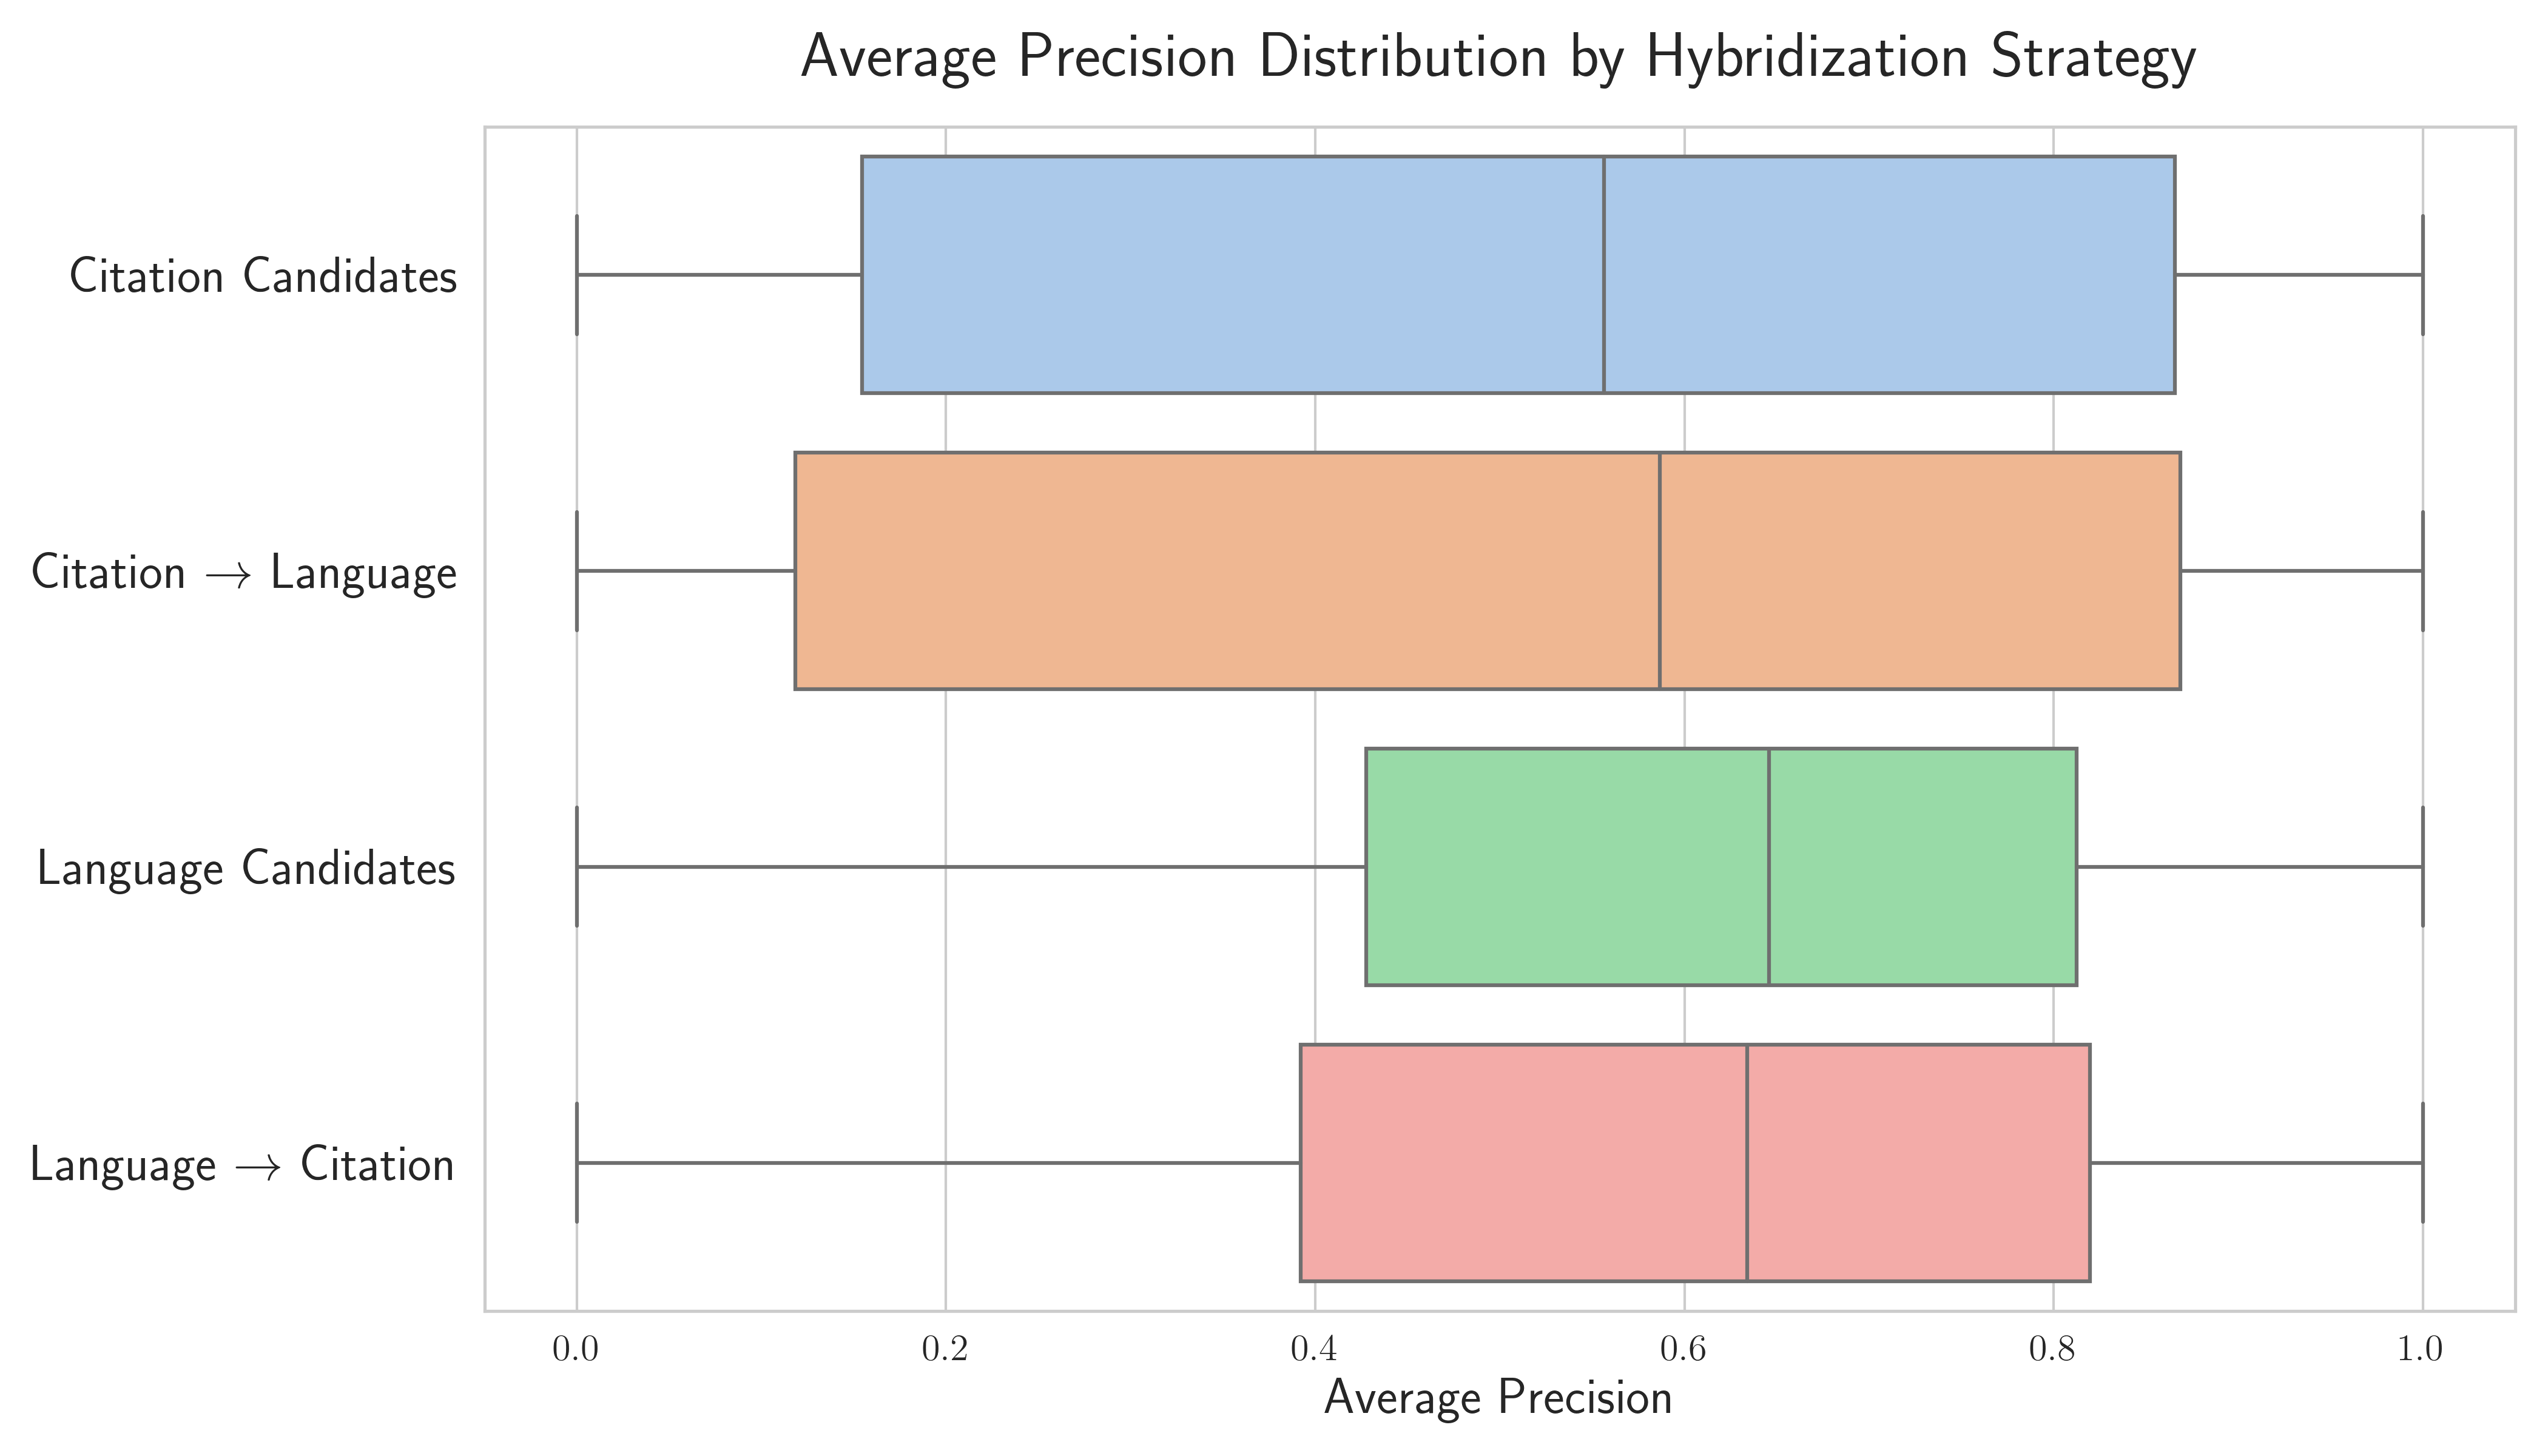
\includegraphics[width=0.9\textwidth]{plots/hybridization_strategies_boxplot.png}
    \caption[Evaluation of Hybridization Strategies]{Comparison of \ac{AP} distributions for the candidate and final recommendations generated by the \ac{C2L} and \ac{L2C} Hybrid Recommenders. The boxplots compile all \ac{AP} scores from the $128,000$ inference runs conducted on the evaluation dataset.
        The vertical lines in each box represent the medians. The corresponding \ac{MAP} values, in order from top to bottom, are $0.505$, $0.522$, $0.594$, and $0.584$. Each of the four distributions has minimum and maximum \ac{AP} values of 0 and 1, respectively. The interquartile ranges, represented by the box widths, are wider when the Citation Recommender is applied first, suggesting a higher variability in performance.}
    \label{fig:hybridization-strategies}
\end{figure}

For the hybrid models, the \ac{L2C} Hybrid Recommender achieves a \ac{MAP} of $0.584$, outperforming the \ac{C2L} Hybrid Recommender's score of $0.522$.
Thus, applying the Language Recommender first for candidate selection and the Citation Recommender second for re-ranking yields a higher \ac{MAP} than the reverse order.
Additionally, the variability in \ac{MAP} for the \ac{C2L} order is much greater than for the \ac{L2C} order, pointing to a higher risk and variability in performance with the \ac{C2L} approach.
In particular, $35.86\%$ of the \ac{AP} scores for the \ac{C2L} Hybrid Recommender are worse than the Null model's \ac{MAP} of $0.384$. In contrast, for the \ac{L2C} Hybrid Recommender, only $24.54\%$ fall short of the Null model's performance.

Comparing candidate and final rankings, only the \ac{C2L} Hybrid Recommender benefits from re-ranking with a \ac{MAP} increase of $0.017$, while the \ac{L2C} Hybrid Recommender experiences a \ac{MAP} decline of $0.010$.
This suggests that, on average, the quality of recommendations generated by the Language Recommender deteriorates upon re-ranking by the Citation Recommender.
Therefore, language models provide valuable information for paper recommendations beyond what global document characteristics and citation-based features offer. The reverse does not hold true.
In this way, the performance gap between the final rankings narrows compared to that of the candidate rankings.


\subsubsection*{Hybridization Strategies by Language Model}

\Cref{fig:hybridization-strategies-by-language-model} takes a more granular perspective than \Cref{fig:hybridization-strategies} by comparing the \ac{MAP} scores stratified by hybridization strategy and language model.
This figure provides additional information beyond \Cref{fig:language-models-feature-weights-heatmap-c2l} by including the reverse \ac{L2C} order as well.
Moreover, the focus of \Cref{fig:hybridization-strategies-by-language-model} is more on the comparison between hybridization strategies rather than between language models.

\begin{figure}[htb!]
    \centering
    \includegraphics[width=\textwidth]{plots/hybridization_strategies_by_language_model_stripplot.png}
    \caption[Evaluation of Hybridization Strategies by Language Model]{Evaluation of hybridization strategies segmented by language model. The colored dots depict the \ac{MAP} values for both \ac{C2L} and \ac{L2C} in their candidate and final recommendations. Except for TF-IDF, all language models enhance the initial recommendations from the Citation Recommender through re-ranking. In the \ac{L2C} order, the impact of re-ranking differs depending on the language model. In every instance, the \ac{L2C} Hybrid Recommender surpasses the performance of the \ac{C2L} Hybrid Recommender. The peak \ac{MAP} value of $0.660$ is attained with the Language Recommender candidates using the SciBERT language model.}
    \label{fig:hybridization-strategies-by-language-model}
\end{figure}

Across all language models, the \ac{L2C} Hybrid Recommender consistently performs better than the \ac{C2L} Hybrid Recommender. Similar to \Cref{fig:language-models-feature-weights-heatmap-c2l}, the improvements are most pronounced for the SciBERT model, where the \ac{L2C} Hybrid Recommender achieves a \ac{MAP} of $0.626$ compared to $0.539$ for the \ac{C2L} Hybrid Recommender. The smallest difference is again observed for the Longformer model, where the \ac{L2C} Hybrid Recommender achieves a \ac{MAP} of $0.542$ compared to $0.514$ for the \ac{C2L} counterpart.

In contrast to the rather uniform behavior for the \ac{C2L} Hybrid Recommender where only the TF-IDF model stands out by decreasing the recommendation performance through re-ranking, the picture for the \ac{L2C} Hybrid Recommender is more diverse.
Top-performing language models like SciBERT, TF-IDF, BERT, and BM25 do not benefit from re-ranking by the Citation Recommender where the \ac{MAP} decline is largest for TF-IDF ($0.628$ to $0.555$) followed by SciBERT ($0.660$ to $0.626$).
Conversely, the lower-performing Longformer, GloVe, FastText, and Word2Vec models experience an uptick in \ac{MAP} post re-ranking with Longformer seeing the largest improvement ($0.524$ to $0.542$).
Thus, while the final recommendations become more similar in \ac{MAP} than the candidate recommendations, it is also notable that the performance of the \ac{L2C} Recommender levels out across different language models.


\subsubsection*{Recommendation Diversity}

As detailed in \Cref{sec:arxiv-labels}, recommendation diversity serves as a secondary metric - beyond \ac{MAP} - to quantify the degree of interdisciplinarity in recommendations.
As recommendation diversity is not affected by the re-ranking process, it is computed for the candidate rankings only.

\Cref{tab:diversity} compares the diversity of candidate recommendations by the Citation and Language Recommenders which correspond to the diversity of the \ac{C2L} and \ac{L2C} Hybrid Recommenders, respectively.
The Language Recommender typically produces more varied recommendations, with a mean of $13.4$ unique labels compared to the Citation Recommender's $9.1$. Both distributions are slightly right-skewed, as evidenced by medians of $13.0$ and $8.0$, respectively.

\begin{table}[htb!]
    \centering
    \begin{tabular}{lcc}
        \toprule
        \textbf{Statistic} & \textbf{Citation $\rightarrow$ Language} & \textbf{Language $\rightarrow$ Citation} \\
        \midrule
        Mean               & 9.1                                      & 13.4                                     \\
        Standard Deviation & 2.6                                      & 3.7                                      \\
        Minimum            & 3.0                                      & 4.0                                      \\
        1st Quartile       & 8.0                                      & 11.0                                     \\
        Median             & 8.0                                      & 13.0                                     \\
        3rd Quartile       & 9.0                                      & 16.0                                     \\
        Maximum            & 24.0                                     & 28.0                                     \\
        \bottomrule
    \end{tabular}
    \caption[Comparison of Recommendation Diversity]{Summary statistics for the recommendation diversity of the \ac{C2L} and \ac{L2C} Hybrid Recommenders. The Language Recommender typically generates more interdisciplinary recommendations across a broader set of categories compared to the Citation Recommender. As the distribution for the Citation Recommender is more closely centered around its median, the number of research fields in its recommendations is more consistent than that of the Language Recommender.}
    \label{tab:diversity}
\end{table}

The spread of unique labels in the Language Recommender's distribution is wider, as indicated by its larger standard deviation ($3.7$ compared to $2.6$)
and its broader interquartile range ($5.0$ versus $1.0$). Both distributions signify outliers in both directions, with the Citation Recommender's range spanning from $3.0$ to $24.0$ and the Language Recommender's range from $4.0$ to $28.0$.

In conclusion, the Language Recommender excels by providing not only more relevant recommendations on average (\Cref{fig:hybridization-strategies}), but also by suggesting papers from a broader array of categories (\Cref{tab:diversity}) than the Citation Recommender.
Whereas the variability of the Language Recommender's \ac{MAP} scores is lower than the variability of the Citation Recommender leading to more robust recommendations, the inverse is true for the recommendation diversity with the Citation Recommender producing more consistent results.
